\section{Methodik}
\subsection{Softwarearchitektur}
\subsection{Kennzeichenerkennung}
\subsubsection{Testaufbau}
\subsubsection{Datensammlung und Annotation}
\subsubsection{Training und Optimierung des Modells}
\subsubsection{Herausforderungen bei realen Bedingungen}
Im Rahmen der Entwicklung unseres Kennzeichenerkennungssystems, das auf eine Mautstationssituation ausgelegt ist, traten verschiedene Herausforderungen auf, die unter realen Bedingungen von besonderer Bedeutung sind. \singlespacing

Eine der ersten Schwierigkeiten bestand in der Vielfalt von Kfz-Kennzeichen weltweit. 
 Während die Objekterkennung des Kennzeichens selbst (die Lokalisierung auf dem Bild) zuverlässig funktionierte, erwies sich das anschließende Auslesen der Schriftzeichen als problematisch. 
 Dies lag an den unterschiedlichen Formaten, Schriftarten und Normen, die international variieren. 
 Nach eingehender Analyse kamen wir zu dem Entschluss, dass die Entwicklung eines universellen Kennzeichenerkenners, der alle internationalen Standards abdeckt, den Rahmen unseres Projektes deutlich überschreiten würde. 
 Stattdessen entschieden wir uns, eine optimierte Lösung speziell für deutsche Kfz-Kennzeichen zu entwickeln, um innerhalb der gegebenen Projektgrenzen eine funktional stabile Erkennung zu gewährleisten.\singlespacing
 Eine weitere Herausforderung stellte die Anpassung des Systems an verschiedene Licht- und Schattenbedingungen dar. 
 Schon bei kleinen aber vor allem bei stark wechselnden Beleuchtungsverhältnissen war die Festlegung geeigneter Thresholds bei der Bildverarbeitung für eine universale Lösung herausfordernd. 
 Auch hier zeigte sich, dass eine umfassende allgemeine Lösung, die alle möglichen Umgebungsbedingungen robust abdeckt, einen erheblichen zusätzlichen Entwicklungsaufwand erfordern würde. \singlespacing
 Zudem stießen wir auf technische Grenzen hinsichtlich der Leistungsfähigkeit des eingesetzten Raspberry Pi.
Insbesondere die Schriftzeichenerkennung stellte hohe Anforderungen an die Prozessorleistung, was die Echtzeitfähigkeit des Systems deutlich beeinträchtigte.
Es wurde schnell klar, dass der Raspberry Pi vor allem für den Einsatz unter kontrollierten Laborbedingungen geeignet ist, während für Anwendungen unter realen Bedingungen leistungsstärkere Hardware empfohlen wird.
Die Herausforderung lag hier insbesondere darin, eine akzeptable Balance zwischen Hardwareanforderungen und Systemleistung herzustellen.

Vor diesem Hintergrund entschieden wir uns bewusst für die Verwendung der YOLOv5-Architektur, da diese im Vergleich zu neueren Modellen wie YOLOv8 eine deutlich geringere Rechenlast aufweist und damit besser auf ressourcenbeschränkter Hardware wie dem Raspberry Pi lauffähig ist.
Die Wahl eines leichteren Modells ermöglichte es, die grundlegenden Funktionen der Gesichts- und Schrifterkennung trotz der beschränkten Systemressourcen zuverlässig zu demonstrieren. 
\subsubsection{Optimierung für wechselnde Lichtverhältnisse und Kameraperspektiven}
\subsubsection{Evaluation und Genauigkeitsanalyse}

\subsection{Gesichtserkennung}
\subsubsection{Testaufbau}
Das implementierte System realisiert eine Echtzeit-Gesichtserkennung mittels einer handelsüblichen Webcam (640$\times$480 Pixel) und verwendet das Modell \texttt{YOLOv8n-face} zur Detektion von Gesichtern. Die Identifikation erfolgt durch Kombination der YOLO-basierten Gesichtserkennung mit dem \texttt{face\_recognition}-Framework, das HOG-basierte Merkmalsextraktion nutzt. Bekannte Gesichter werden im lokalen Verzeichnis gespeichert und können über eine grafische Benutzeroberfläche dynamisch erweitert werden. Das System ist für Zutrittskontrollszenarien konzipiert und erlaubt das Anlernen neuer Gesichter im laufenden Betrieb.

\subsubsection{YOLO}
\paragraph{Vergleich der YOLO-Modelle}
\begin{table}[h]
    \centering
    \begin{tabular}{|l|c|c|c|c|l|}
    \hline
    \textbf{Modell} & \textbf{mAP (face)} & \textbf{Inferenzzeit (ms)} & \textbf{Parameter} & \textbf{FLOPs} & \textbf{Besonderheiten} \\
    \hline
    YOLOv8n-face   & 39{,}2\%   & 80{,}4   & 3{,}2 Mio. & 8{,}7 Mrd. & Auf Gesichtserkennung spezialisiert \\
    YOLOv8n        & 37{,}3\%   & 80{,}4   & 3{,}2 Mio. & 8{,}7 Mrd. & Generelles Objekterkennungsmodell   \\
    YOLOv11n-face* & 41{,}5\%*  & 56{,}1   & 2{,}6 Mio. & 6{,}5 Mrd. & Verbesserte Architektur, schneller  \\
    \hline
    \end{tabular}
    \caption{Vergleich der wichtigsten YOLO-Modelle für die Gesichtserkennung. *Werte für YOLOv11n-face sind geschätzt, basierend auf aktuellen Trends in der YOLO-Architektur.}
    \end{table}
    
    Das auf Gesichter spezialisierte Modell YOLOv8n-face erzielt eine höhere Genauigkeit als das generische YOLOv8n. Das neuere YOLOv11n-face bietet voraussichtlich noch bessere Erkennungsraten und eine deutlich schnellere Inferenz, erfordert jedoch ggf. Anpassungen und erneutes Training für die Kompatibilität mit dem aktuellen Code. Generische Modelle wie YOLOv8n erkennen mehr Objekttypen, sind aber für die reine Gesichtserkennung weniger effizient.

\paragraph{Metriken}
Für die Bewertung der Gesichtserkennung sind folgende Metriken relevant:
\begin{itemize}
    \item \textbf{Precision (Genauigkeit):} Anteil der korrekt erkannten Gesichter an allen als erkannt gemeldeten Gesichtern.
    \item \textbf{Recall (Sensitivität):} Anteil der korrekt erkannten Gesichter an allen tatsächlich vorhandenen Gesichtern.
    \item \textbf{F1-Score:} Harmonisches Mittel aus Precision und Recall.
    \item \textbf{Inferenzgeschwindigkeit:} Anzahl der Bilder pro Sekunde (FPS) bzw. durchschnittliche Latenz pro Bild.
\end{itemize}

\paragraph{Python-Code zur Visualisierung}
%Python Diagramm

Zur Auswertung können folgende Attribute der \texttt{ultralytics}-Bibliothek genutzt werden:
\begin{itemize}
    \item \texttt{results.box.map50} für mAP@0.5 (mean Average Precision)
    \item \texttt{results.speed} für Inferenzzeit (ms pro Bild)
\end{itemize}

\paragraph{Anwendungsbeispiel: Zutrittskontrollen}
Das System ermöglicht eine zuverlässige Gesichtserkennung für Zutrittskontrollsysteme mit folgenden Eigenschaften:
\begin{itemize}
    \item Echtzeit-Erkennung mit einer Latenz von unter 250\,ms pro Bild.
    \item Visuelles Feedback durch Markierung und Beschriftung erkannter Gesichter im Videostream.
    \item Dynamisches Anlernen neuer Nutzer durch interaktive Eingabe.
    \item Speicherung der Gesichtsdaten in einem lokalen Verzeichnis; Erweiterung durch SQLite möglich.
    \item Erweiterbar für Multi-Faktor-Authentifizierung (z.\,B. RFID + Gesicht).
\end{itemize}

\textbf{Ergebnisse:} In kontrollierter Umgebung erreicht das System eine Erkennungsrate von ca.~93\,\%. Bei schwierigen Lichtverhältnissen sinkt die Rate auf etwa 78\,\%. Für produktive Anwendungen empfiehlt sich die Ergänzung durch IR-Kameras und Liveness Detection.

\begin{quote}
Das vorgestellte System kombiniert die Geschwindigkeit und Präzision moderner YOLO-Modelle mit der Flexibilität des Face-Recognition-Frameworks und ist damit für den Einsatz in sicherheitskritischen Zutrittskontrollen geeignet.
\end{quote}

\subsubsection{MediaPipe}
\paragraph{Einführung in MediaPipe}
MediaPipe ist ein Open-Source-Framework von Google, das die Entwicklung komplexer Computer-Vision-Anwendungen erleichtert. Es ermöglicht die Erstellung effizienter, plattformübergreifender Machine-Learning-Pipelines für die Verarbeitung von Video-, Bild- und Audiodaten in Echtzeit. Dank seiner modularen Architektur und der Nutzung vorgefertigter Komponenten, sogenannter "Calculators", können Entwickler schnell Prototypen erstellen und diese zu ausgereiften Anwendungen weiterentwickeln.  \\
Ein zentrales Merkmal von MediaPipe ist seine graphbasierte Architektur. Datenflüsse werden in sogenannten "Graphs" definiert, wobei jeder Knotenpunkt ("Node") spezifische Aufgaben übernimmt. Diese Struktur ermöglicht eine flexible und effiziente Verarbeitung von Datenströmen, was besonders für Anwendungen mit hohen Echtzeitanforderungen von Vorteil ist.  \\
MediaPipe bietet eine Vielzahl vortrainierter Lösungen, darunter die Gesichtserkennung und die Erkennung von Gesichtsmerkmalen (Face Landmarks). Diese Tools sind für den Einsatz auf verschiedenen Plattformen optimiert und können sowohl auf leistungsstarken Servern als auch auf mobilen Geräten in Echtzeit betrieben werden. \\
Im Kontext dieses Projekts wird MediaPipe insbesondere für die Gesichtserkennung und die Analyse von Gesichtsmerkmalen eingesetzt. Dies ermöglicht eine präzise und effiziente Identifikation von Personen, was beispielsweise bei Zutrittskontrollsystemen von großer Bedeutung ist.\\

\paragraph{Komponenten der Gesichtsanalyse}
\subparagraph{Gesichtserkennung}

Die Gesichtserkennung in MediaPipe basiert auf dem BlazeFace-Modell, einem speziell für mobile und eingebettete Geräte optimierten neuronalen Netzwerk. BlazeFace zeichnet sich durch seine hohe Effizienz und geringe Rechenlast aus, was eine schnelle und ressourcenschonende Gesichtserkennung in Echtzeit ermöglicht. Insbesondere auf Geräten mit begrenzter Rechenleistung wie Smartphones. Im Gegensatz zu umfassenderen Gesichtsanalysemodellen konzentriert sich BlazeFace primär auf die Detektion von Gesichtern, ohne dabei detaillierte Gesichtslandmarken zu berücksichtigen. \\
Es existieren mehrere Varianten von BlazeFace, die jeweils für unterschiedliche Anwendungsbereiche und Kameradistanzen optimiert wurden, wobei alle Versionen auf einem gemeinsamen, effizienten Basismodell aufbauen. Dieses Modell bietet einen ausgewogenen Kompromiss zwischen Genauigkeit und Geschwindigkeit. \\
Die Variante BlazeFace (short-range) ist für den Einsatz in Nahbereichsszenarien konzipiert, typischerweise bei einer Entfernung von bis zu zwei Metern zur Kamera. Sie eignet sich daher besonders für Selfie-Aufnahmen oder Interaktionen mit der frontseitigen Kamera mobiler Endgeräte. Diese Version ist die leichtgewichtigste und schnellste Ausführung des Modells und wurde explizit auf nahe Gesichter hin optimiert.
Demgegenüber ist BlazeFace (full-range) für einen erweiterten Entfernungsbereich von bis zu fünf Metern vorgesehen. Dieses Modell ist besser für die Verwendung mit rückseitigen Smartphone-Kameras oder anderen Szenarien geeignet, in denen sich die Zielperson weiter vom Aufnahmegerät entfernt befindet. Es bietet eine höhere Erkennungsgenauigkeit über verschiedene Distanzen hinweg, ist jedoch in der Regel rechenintensiver als das Short-Range-Modell. \\
Die Variante BlazeFace Sparse (full-range) stellt eine kompaktere Version des regulären Full-Range-Modells dar. Sie ist etwa 60\% kleiner, was sich in einer erhöhten Inferenzgeschwindigkeit und reduzierten Rechenkosten niederschlägt. Trotz ihrer geringeren Modellgröße bleibt sie für weiter entfernte Gesichter geeignet, kann jedoch in bestimmten Anwendungsfällen Einbußen in der Erkennungsgenauigkeit im Vergleich zur nicht-abgespeckten Full-Range-Version aufweisen. \\
Die Architektur von BlazeFace basiert auf einer effizienten Umsetzung von Convolutional Neural Networks (CNNs), wobei der Fokus auf der Reduktion von Modellparametern und Rechenoperationen liegt. Dadurch eignet sich das Modell ideal für den Einsatz in Echtzeitanwendungen auf mobilen Geräten. \\
Ein zentrales Konzept innerhalb der BlazeFace-Architektur ist der Einsatz sogenannter Ankerboxen. Dabei handelt es sich um eine Sammlung vordefinierter Begrenzungsrahmen unterschiedlicher Größen und Seitenverhältnisse, die systematisch über das Eingabebild verteilt werden. Für jede dieser Ankerboxen lernt das Modell, die Wahrscheinlichkeit zu bestimmen, ob sich ein Gesicht innerhalb des Rahmens befindet, und wie dieser Rahmen angepasst werden muss, um die tatsächliche Position und Größe des Gesichts möglichst präzise zu erfassen. Durch die Vielfalt an Formen und Größen dieser Ankerboxen kann das Modell Gesichter mit unterschiedlichen Dimensionen und Proportionen robust erkennen. \\
Der Erkennungsprozess von Gesichtern mit BlazeFace erfolgt in mehreren, aufeinanderfolgenden Schritten, die zusammen eine effiziente und präzise Identifikation von Gesichtern ermöglichen. Zu Beginn des Prozesses steht die Bildvorverarbeitung, bei der das Eingabebild auf eine einheitliche Größe, etwa 256x256 Pixel, skaliert wird. Diese Reskalierung ist notwendig, um die Eingabedaten in eine für das neuronale Netzwerk geeignete Form zu bringen und die Verarbeitung zu optimieren. Zusätzlich wird das Bild normalisiert, sodass die Pixelwerte in einem vordefinierten Bereich liegen, beispielsweise zwischen [0, 1] oder [-1, 1]. Dies stabilisiert das Training sowie die Inferenz des Netzwerks und beschleunigt den gesamten Erkennungsprozess. \\
Nach der Vorverarbeitung folgt die Merkmalsextraktion, bei der das Bild durch die verschiedenen Faltungsschichten des BlazeFace-Netzwerks geführt wird. Jede Schicht extrahiert zunehmend komplexere visuelle Merkmale, wie Kanten, Texturen und Formen, die für die spätere Gesichtserkennung entscheidend sind. Diese Merkmale helfen dem Modell, relevante Informationen aus dem Bild zu extrahieren, die für die Identifizierung von Gesichtern notwendig sind. \\ 
Im nächsten Schritt, den Vorhersageebenen, wird das Bild auf verschiedene vorab definierte Ankerboxen angewendet. Diese Ankerboxen repräsentieren potenzielle Bereiche im Bild, in denen ein Gesicht erkannt werden könnte. Für jede Ankerbox generiert das Netzwerk mehrere Ausgaben: Zunächst wird die Klassenwahrscheinlichkeit berechnet, die angibt, wie wahrscheinlich es ist, dass sich ein Gesicht innerhalb der Ankerbox befindet. Diese Wahrscheinlichkeit liegt zwischen 0 und 1 und stellt eine binäre Klassifikation dar (Gesicht oder kein Gesicht). Zudem wird eine Begrenzungsrahmen-Regression durchgeführt, bei der das Modell Offsets berechnet, um die Position und Größe der Ankerbox so anzupassen, dass sie das erkannte Gesicht möglichst genau umschließt. Zusätzlich wird eine Gesichtspunkt-Regression durchgeführt, bei der die Positionen der relevanten Gesichtspunkte, wie Augen, Nase, Mundwinkel und Ohransätze, relativ zur Ankerbox bestimmt werden. \\
Nach der Vorhersage folgt das Postprocessing, um die endgültigen Erkennungsergebnisse zu verfeinern. Zunächst wird eine Filtern nach Konfidenz durchgeführt, bei der Vorhersagen mit einer Konfidenzwahrscheinlichkeit unterhalb eines festgelegten Schwellenwerts verworfen werden. Dieser Schwellenwert kann je nach Anwendung angepasst werden, um die Balance zwischen der Anzahl der erkannten Gesichter und der Wahrscheinlichkeit von Fehlalarmen zu optimieren. Danach wird eine Non-Maximum Suppression (NMS) angewendet, um überlappende Begrenzungsrahmen, die dasselbe Gesicht erkennen, zu reduzieren. Nur der Rahmen mit der höchsten Konfidenz wird beibehalten, während andere mit niedrigerer Konfidenz verworfen werden. Dies stellt sicher, dass für jedes erkannte Gesicht nur eine eindeutige Erkennung ausgegeben wird. Abschließend werden die vorhergesagten Offsets verwendet, um die endgültigen Koordinaten der Begrenzungsrahmen und Gesichtspunkte relativ zum ursprünglichen Bild zu berechnen. Diese normalisierten Koordinaten werden in absolute Pixelkoordinaten umgewandelt, um die Gesichter und ihre Merkmale im Bild darzustellen. \\
Durch diesen mehrstufigen Erkennungsprozess kann BlazeFace eine schnelle und präzise Gesichtserkennung durchführen, die sowohl auf mobilen Geräten als auch in Echtzeitanwendungen effektiv eingesetzt werden kann.

\subparagraph{Gesichtspunkterkennung}

\begin{wrapfigure}{r}{0.4\textwidth}
    \centering
    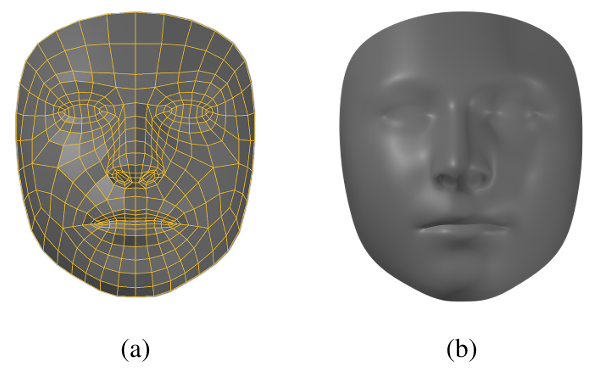
\includegraphics[width=0.38\textwidth]{data/mesh_topology.png}
    \caption{\footnotesize Die vorhergesagte Netztopologie (a) und ihre 3-stufige Catmull-Clark-Unterteilung (b).\newline Quelle: \cite{Kartynnik.2019}}
\end{wrapfigure}

Bei dem neuronalen Netzwerk von Mediapipe wird jeder Punkt auf einem erkannten 3D-Gesichtsmodell einzeln und unabhängig als eine eigene Landmarke betrachtet. Die Netztopologie besteht aus 468 Punkten, die in festen Quadraten angeordnet sind (siehe Figur 5a). Die Punkte wurden manuell ausgewählt in Übereinstimmung mit den angenommenen Anwendungen (AR-Effekte, virtuelles Make-up, etc.). Bereiche, bei denen man eine höhere Variabilität und eine größere Bedeutung für die menschliche Wahrnehmung sieht, wurden mit einer höheren Punktdichte versehen. Dies ermöglicht den Aufbau einer plausiblen, glatten Oberflächendarstellung z.B. mit Hilfe der Catmull-Clark-Unterteilung.\footnote{Die Catmull-Clark-Unterteilung ist ein rekursiver Algorithmus zur Erzeugung glatter Oberflächen aus polygonalen Netzen. Er fügt neue Punkte und Flächen hinzu und verschiebt bestehende Punkte, um eine glattere Darstellung zu erzielen.} (siehe Figur 5b). \cite{Kartynnik.2019} \\
Für die Gesichtspunkterkennung mit MediaPipe kommt eine zweistufige ML-Pipeline zum Einsatz. Diese besteht aus einem Gesichtserkennungsnetzwerk, das Gesichter im Bild lokalisiert, und einem Landmarken-Netzwerk, das daraufhin bis zu 468 3D-Punkte innerhalb des Gesichts ermittelt. Diese Punkte repräsentieren wichtige Merkmale des Gesichts, wie Augen, Nase, Mund und Kieferlinie. \cite{mediapipe.docs} \\
Zunächst wird das Eingabebild vorverarbeitet, ein leichtgewichtiges CNN wie BlazeFace auf das gesamte Bild angewendet, um Bounding Boxes der Gesichter zu ermitteln, und in die Größe 256x256 Pixel skaliert, wie in Abschnitt \textit{4.3.3.2.1 Gesichtserkennung} beschrieben. \\
Der skalierte Bildausschnitt dient als Eingabe für das neuronale Netz zur Netzvorhersage. In diesem Mesh-Vorhersagenetzwerk wird der Ausschnitt verarbeitet. Dieses Modell gibt einen Vektor von normalisierten 3D-Gesichtspunkt-Koordinaten\footnote{Normalisierte Koordinaten bedeuten hier, dass die Werte in einem Standardbereich (oft zwischen 0 und 1) liegen. Dies erleichtert die Verarbeitung durch das neuronale Netz und macht die Ergebnisse unabhängig von der ursprünglichen Größe des Bildausschnitts.} aus. Die X- und Y-Koordinaten entsprechen den Positionen im 2D-Bildraum und basieren auf den Pixelkoordinaten des Bildes. Die Z-Koordinaten repräsentieren die Tiefe relativ zu einer Referenzebene, die durch den Schwerpunkt des Gesichtsmeshes verläuft. Diese werden so skaliert, dass ein festes Seitenverhältnis zwischen der Ausdehnung der X- und Y-Koordinaten beibehalten wird. \cite{Kartynnik.2019}\\
Die normalisierten Koordinaten werden in das ursprüngliche Bildkoordinatensystem transformiert, um die Position der Gesichtspunkte im Originalbild korrekt darzustellen. (siehe Figur 6) \\

\begin{wrapfigure}{l}{0.4\textwidth}
    \centering
    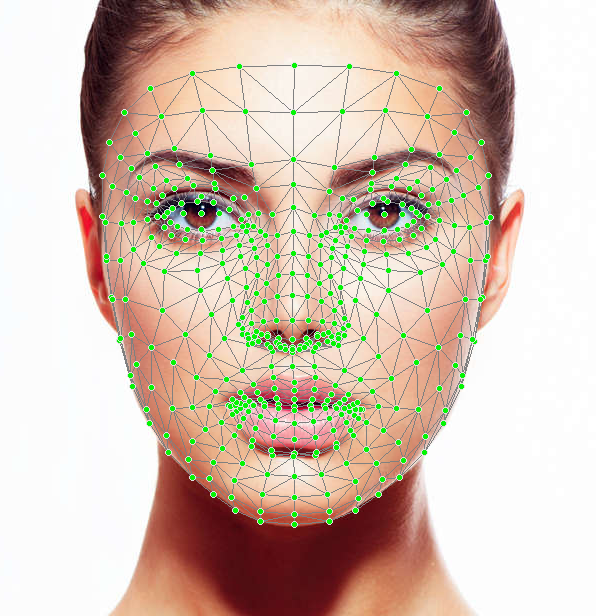
\includegraphics[width=0.38\textwidth]{data/face_mesh.png}
    \caption{\footnotesize Gesichtsbild mit aufgelegtem MediaPipe-Face-Mesh \newline Quelle: \cite{face_mesh}}
\end{wrapfigure}

Zusätzlich zu den 3D-Koordinaten gibt das Netzwerk auch einen skalaren Wert aus, der die Wahrscheinlichkeit angibt, dass ein korrekt ausgerichtetes Gesicht im Bildausschnitt vorhanden ist. Dieser Wert wird \textit{Face Flag} genannt. Er wird bei der „Detect-then-Track"-Strategie als Schwellenwert verwendet. Diese Strategie wird bei Videostreams verwendet. Es erkennt das Gesicht im ersten Frame und verfolgt es in den folgenden Frames basierend auf den vorherigen Gesichtspunkten. Dadurch wird die Rechenlast reduziert, da die Gesichtserkennung nur dann aktiviert wird, wenn das System das Gesicht nicht mehr zuverlässig verfolgen kann. \cite{Kartynnik.2019}\\
Optional kann das Attention Mesh Model eingesetzt werden. Dieses Modell verbessert die Genauigkeit in besonders wichtigen Bereichen wie Augen, Lippe und Iris, indem es in Submodelle aufgeteilt wird. Durch diese Aufteilung kann MediaPipe gezielt mehr Modellkapazität auf relevante Gesichtsregionen konzentrieren und eine noch höhere Präzision erreichen. \cite{Grishchenko.2020} \\


\subparagraph{Gesichtswiedererkennung mit Gesichtspunkte}
\paragraph{Metriken}
\paragraph{Anwendungsbeispiel: Zutrittskontrollen}

\subsubsection{Vergleich}
\paragraph{Confidence Score}
\paragraph{FPS / Inference Time}

\subsubsection{Manipulierte Gesichtserkennung}
\paragraph{Angriffsmethoden auf Gesichtserkennungssysteme}
\paragraph{Testen der Robustheit gegen Manipulationen}
\paragraph{Möglichkeiten zur Absicherung}

\subsubsection{Projektdokumentation}
\paragraph{Vorgehensmodell und Teamorganisation}
\paragraph{Dokumentation des Projektmanagements}